\documentclass[11pt]{article}
\usepackage{amsmath}
\usepackage{graphicx}
\usepackage{float}

% Margins
\topmargin=-0.45in
\evensidemargin=0in
\oddsidemargin=0in
\textwidth=6.5in
\textheight=9.0in
\headsep=0.25in

\title{Comparison between NEK5000 and Xcompact3D}
\author{Gaurav Gupta}
\date{\today}

\begin{document}
\maketitle


\section{Case for Comparison}
Flow over cylinder at $Re=40$ was simulated using NEK5000 and Xcompact3D to compare the codes in terms of accuracy and performance.
The flow properties have been studied by \textbf{Kawaguti (1953)} and \textbf{Taneda (1955)}. The data from the steady flow analysis by Kawaguti
and experiments by Taneda are used for comparison.\\

\noindent Six simulations where performed by varying the number of elements as well as the domain height.

\begin{table}[H]
    \caption{Labels for different simulations.}
    \begin{tabular}{|c|c|}
        \hline
        \textbf{Label} & \textbf{Description}                                                            \\
        \hline
        X3D-LR         & Low resolution simulation using Xcompact3d with a domain height of $16D$        \\
        \hline
        X3D-HR         & High resolution simulation using Xcompact3d with a domain height of $16D$       \\
        \hline
        X3D-H20        & Low resolution simulation using Xcompact3d with a domain height of $20D$        \\
        \hline
        NEK-P6         & Simulation using NEK5000 with a domain height of $16D$ and 5th Order Polynomial \\
        \hline
        NEK-P8         & Simulation using NEK5000 with a domain height of $16D$ and 7th Order Polynomial \\
        \hline
        NEK-H20        & Simulation using NEK5000 with a domain height of $16D$ and 5th Order Polynomial \\
        \hline
    \end{tabular}
\end{table}

\section{Results}
\subsection{Performance}
All the simulations were run on an HPC using 36 cores. We compare the time taken by
each code to compute 1 second of flow i.e.
$$
    \mathbf{\tau} = \frac{\text{Compute Time}}{\text{Simulation Time}}
$$
\begin{table}[H]
    \caption{Performance comparison of the different simulations}
    \begin{tabular}{|c|c|c|c|c|c|}
        \hline
        \textbf{Label} & \textbf{No. of Elements} & \textbf{dt} & \textbf{Simulation Time (s)} & \textbf{Compute Time (Hr)} & $\mathbf{\tau}$ \textbf{(hr/s)} \\
        \hline
        X3D-LR         & 526336                   & 0.00025     & 40                           & 0.7967                     & 0.019917                        \\
        \hline
        X3D-HR         & 657920                   & 0.000125    & 60                           & 5.063                      & 0.084383                        \\
        \hline
        X3D-H20        & 657920                   & 0.00025     & 30                           & 0.8544                     & 0.02848                         \\
        \hline
        NEK-P6         & 7000                     & 0.005       & 60                           & 1.0046                     & 0.01674                         \\
        \hline
        NEK-P8         & 7000                     & 0.005       & 60                           & 5.35                       & 0.089166                        \\
        \hline
        NEK-H20        & 9300                     & 0.005       & 60                           & 1.2163                     & 0.02027                         \\
        \hline
    \end{tabular}
\end{table}
\noindent NEK-P6 has the smallest value of $\mathbf{\tau}$ i.e. it has the best performance among all the simulations.
\newpage
\subsection{Accuracy}
The accuracy of the simulations are tested by comparing four parameters
\begin{itemize}
    \item Drag Coefficient
    \item Velocity Distribution along the x-axis
    \item Length of Twin-vortices
    \item Angular position of flow seperation
\end{itemize}
The values of the following parameters are compared with the results of steady-state numerical computation
of the flow by \textbf{Kawaguti (1953)} which are in good agreement with the experimental results as shown by
\textbf{Taneda (1955)}.

\subsubsection*{Drag Coefficient}
The drag coefficient for a flow over a cylinder at Re=40 is 1.6177.
The closest value of drag coefficient among all the simulation were obtained by all the NEK5000 simulations i.e. 1.921 (18\% Error).
The time evolution of drag coefficient for all the simulations is presented in \textbf{Figure \ref{fig:drag}}.

\begin{figure}[H]
    \centering
    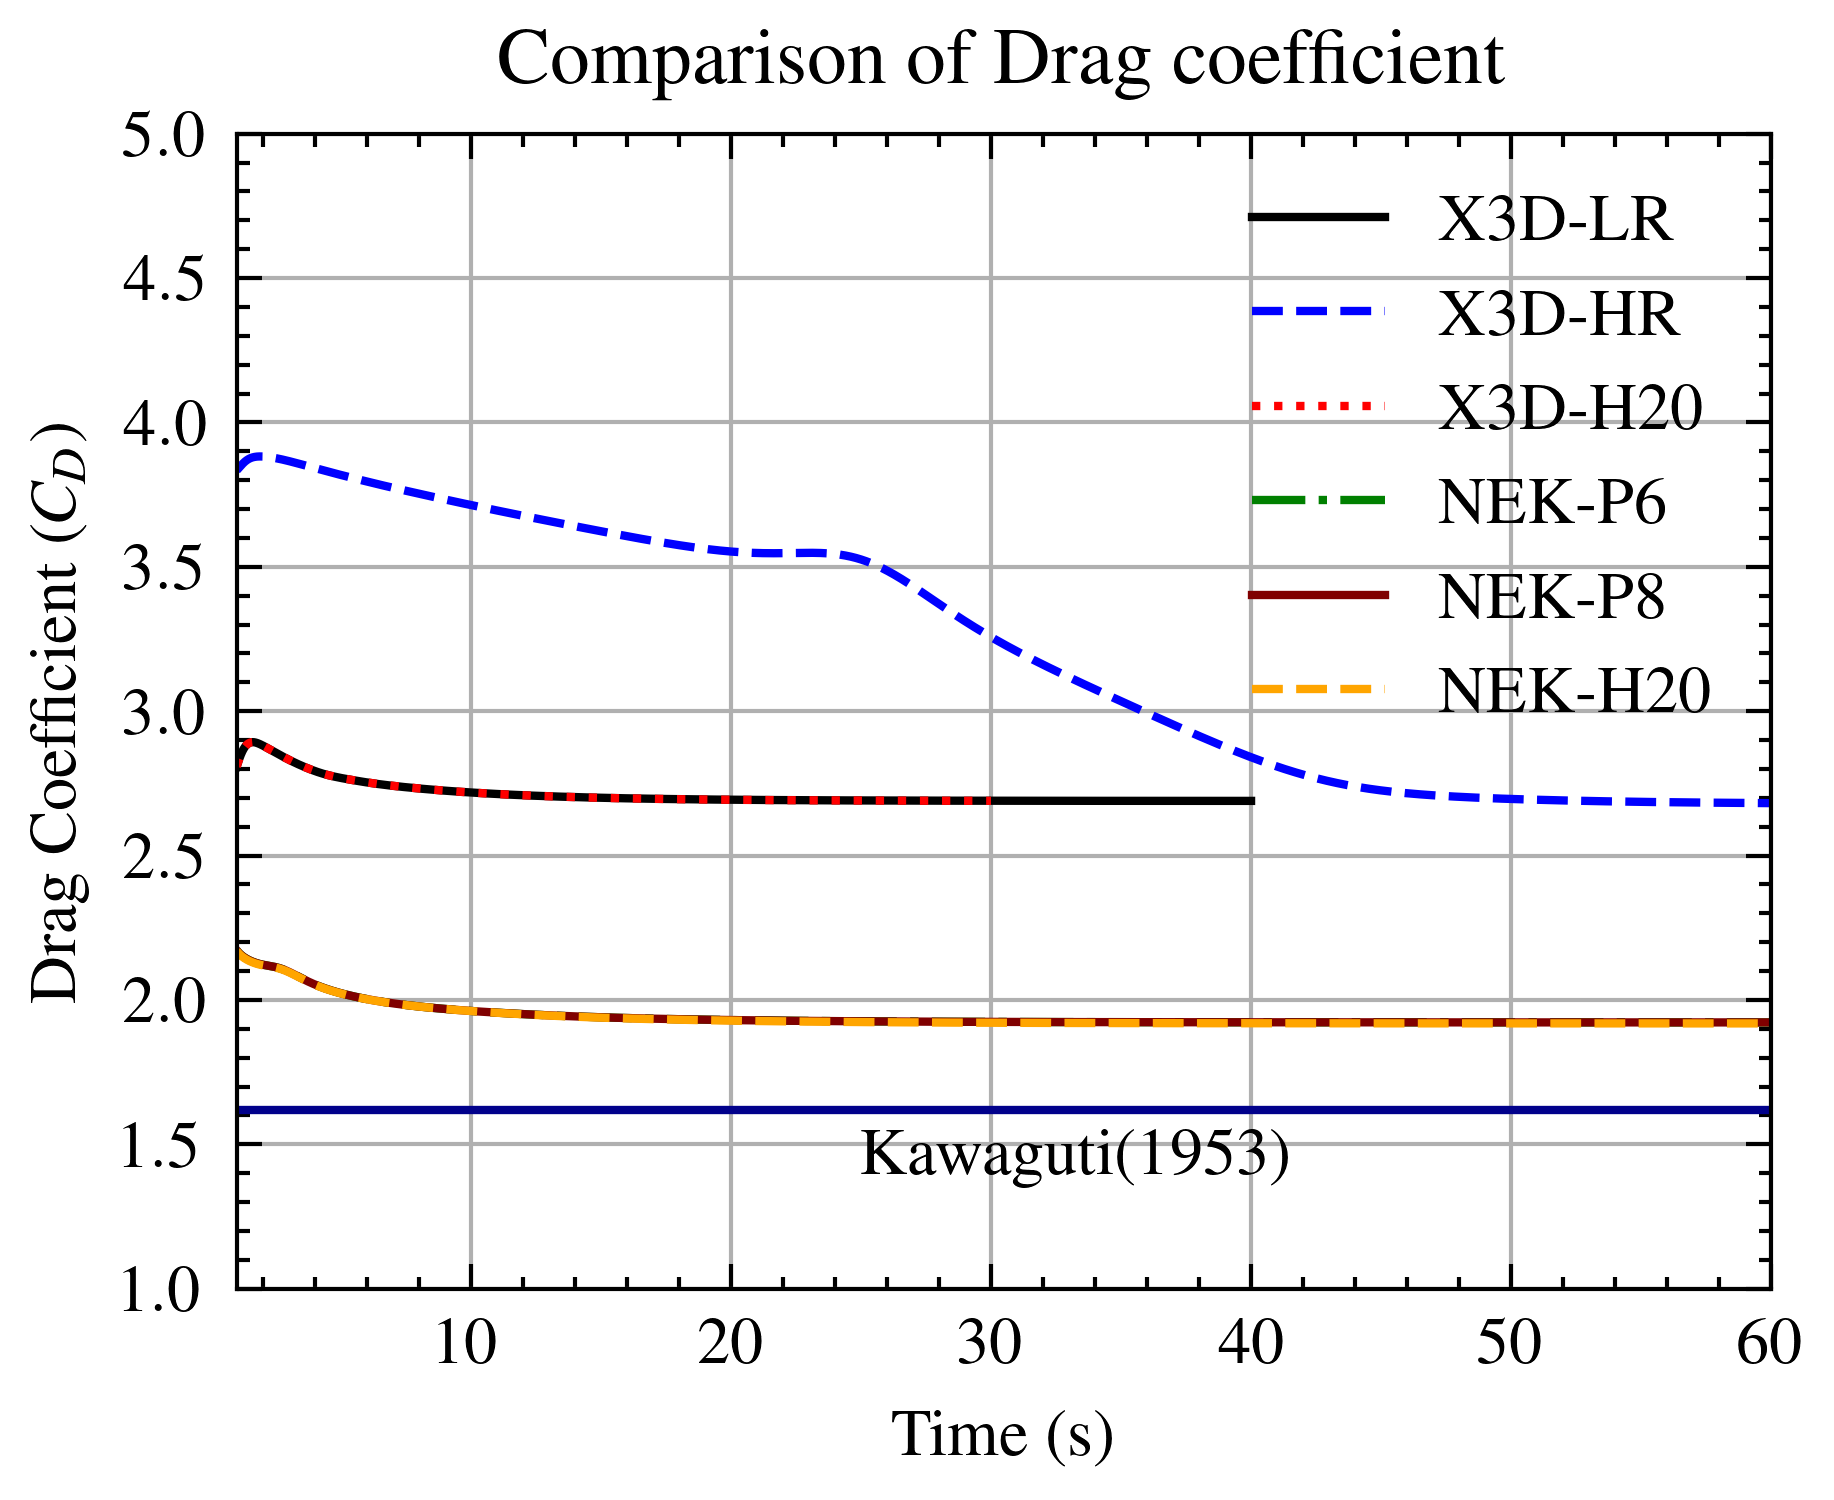
\includegraphics[width=0.7\textwidth]{../drag.png}
    \caption{Time evolution of $C_D$ for the different simulations.}
    \label{fig:drag}
\end{figure}

\noindent We observe that increasing the domain height from $16D$ to $20D$ didn't affect the drag values
as the plot for NEK-P6 and NEK-H20 coincide with each other. The same is also observed with X3D-LR and X3D-H20 cases.

\newpage
\subsubsection*{Velocity Distribution along the X-axis}
The time evolution of the velocity at two points is plotted to find the instant when flow reaches steady-state.
The velocity along X-axis after flow has reached steady state is compared with the results of \textbf{Kawaguti (1953)}.

\begin{figure}[H]
    \centering
    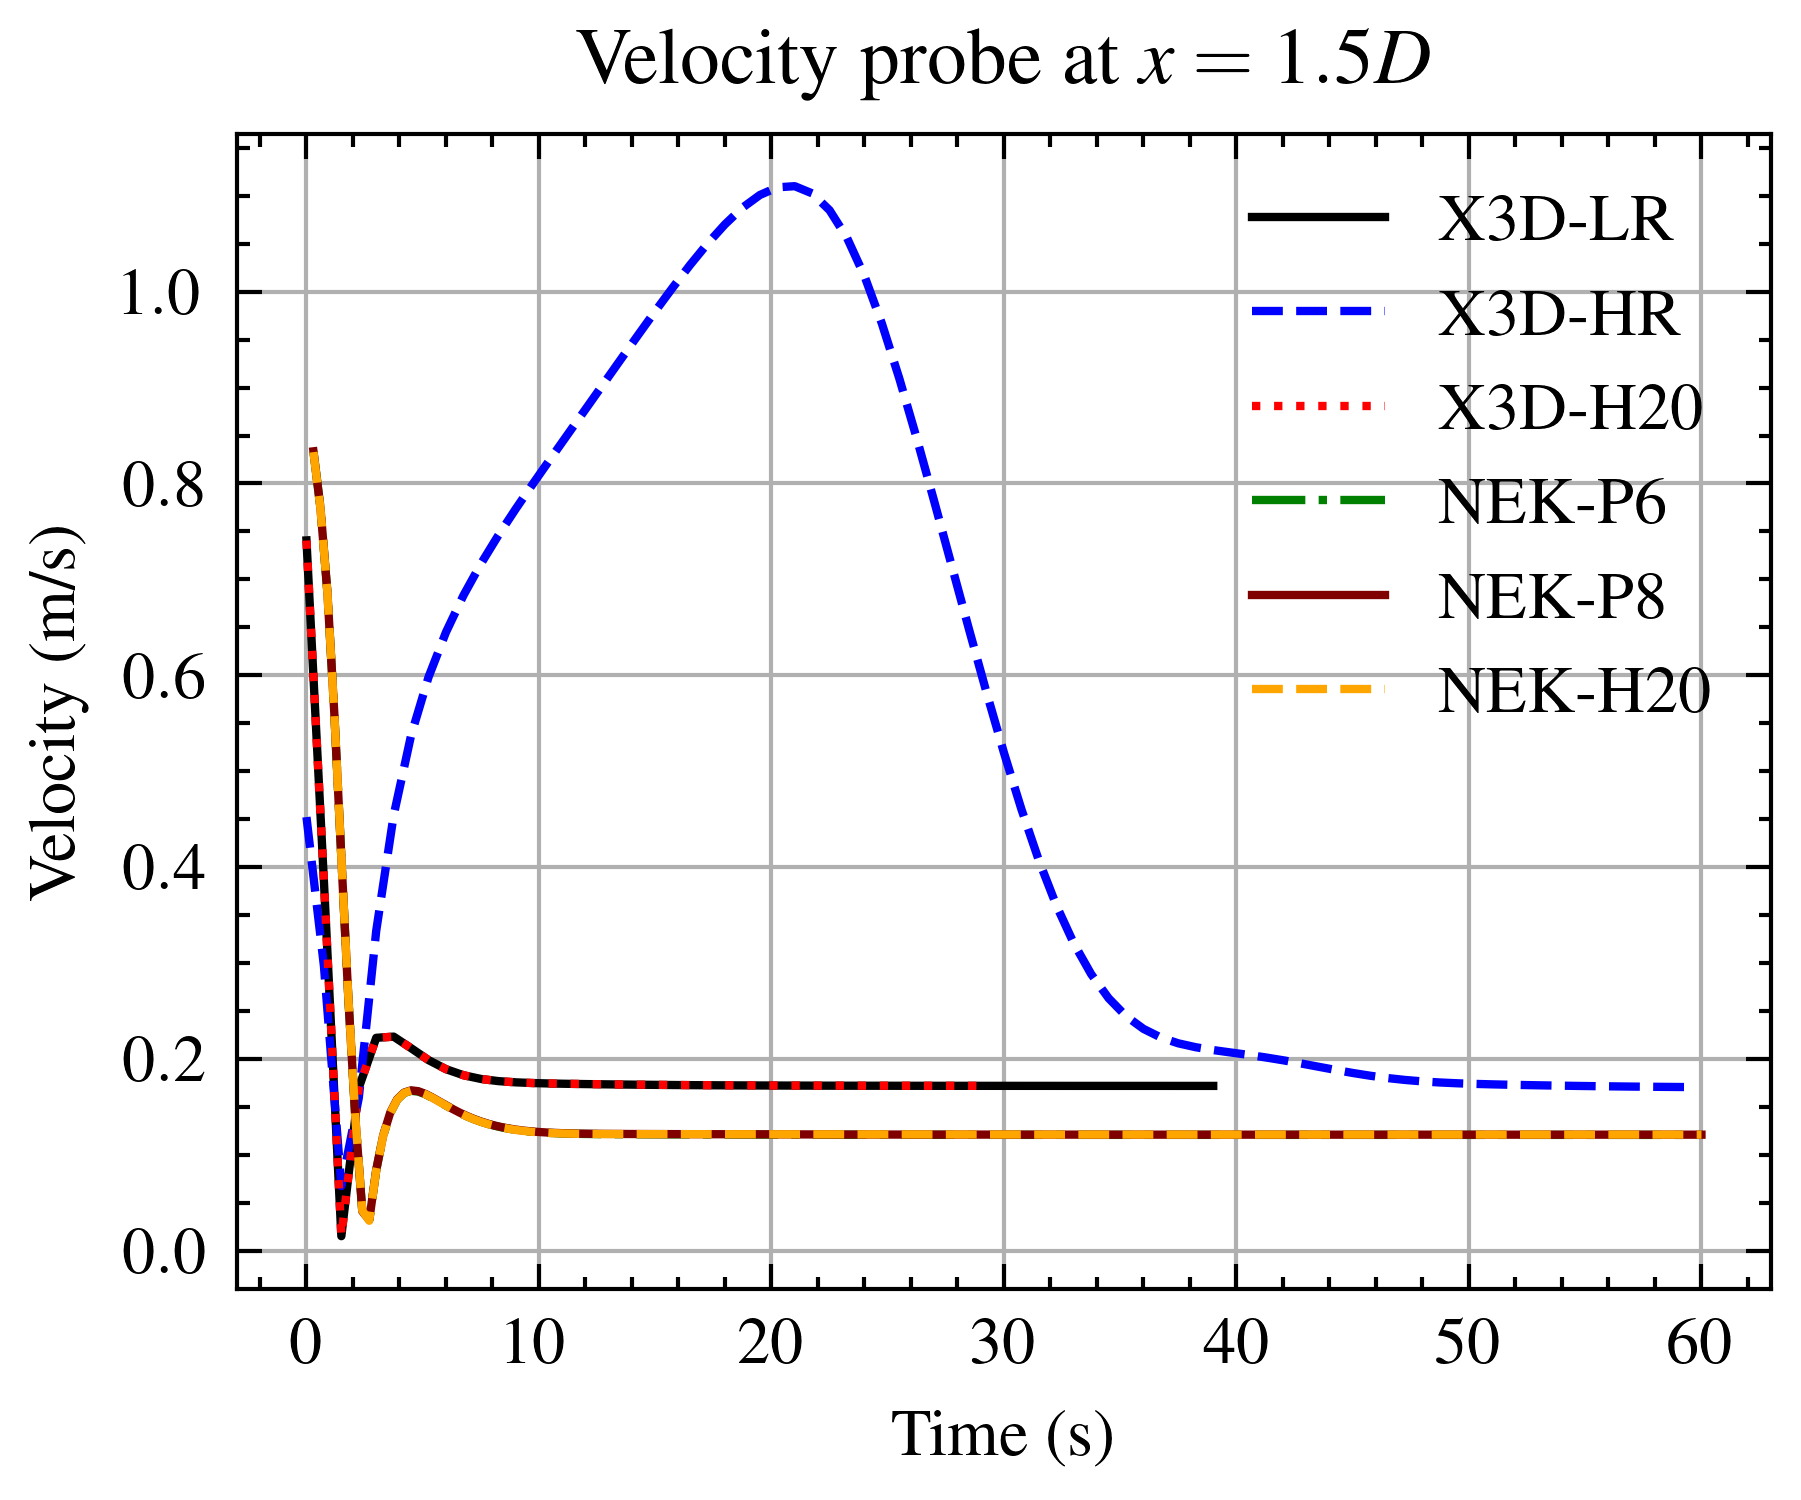
\includegraphics[width=0.55\textwidth]{../ss3.png}
    \caption{Time evolution of velocity magnitude at $x=1.5 D$ for the different simulations.}
    \label{fig:ss3}
\end{figure}

\begin{figure}[H]
    \centering
    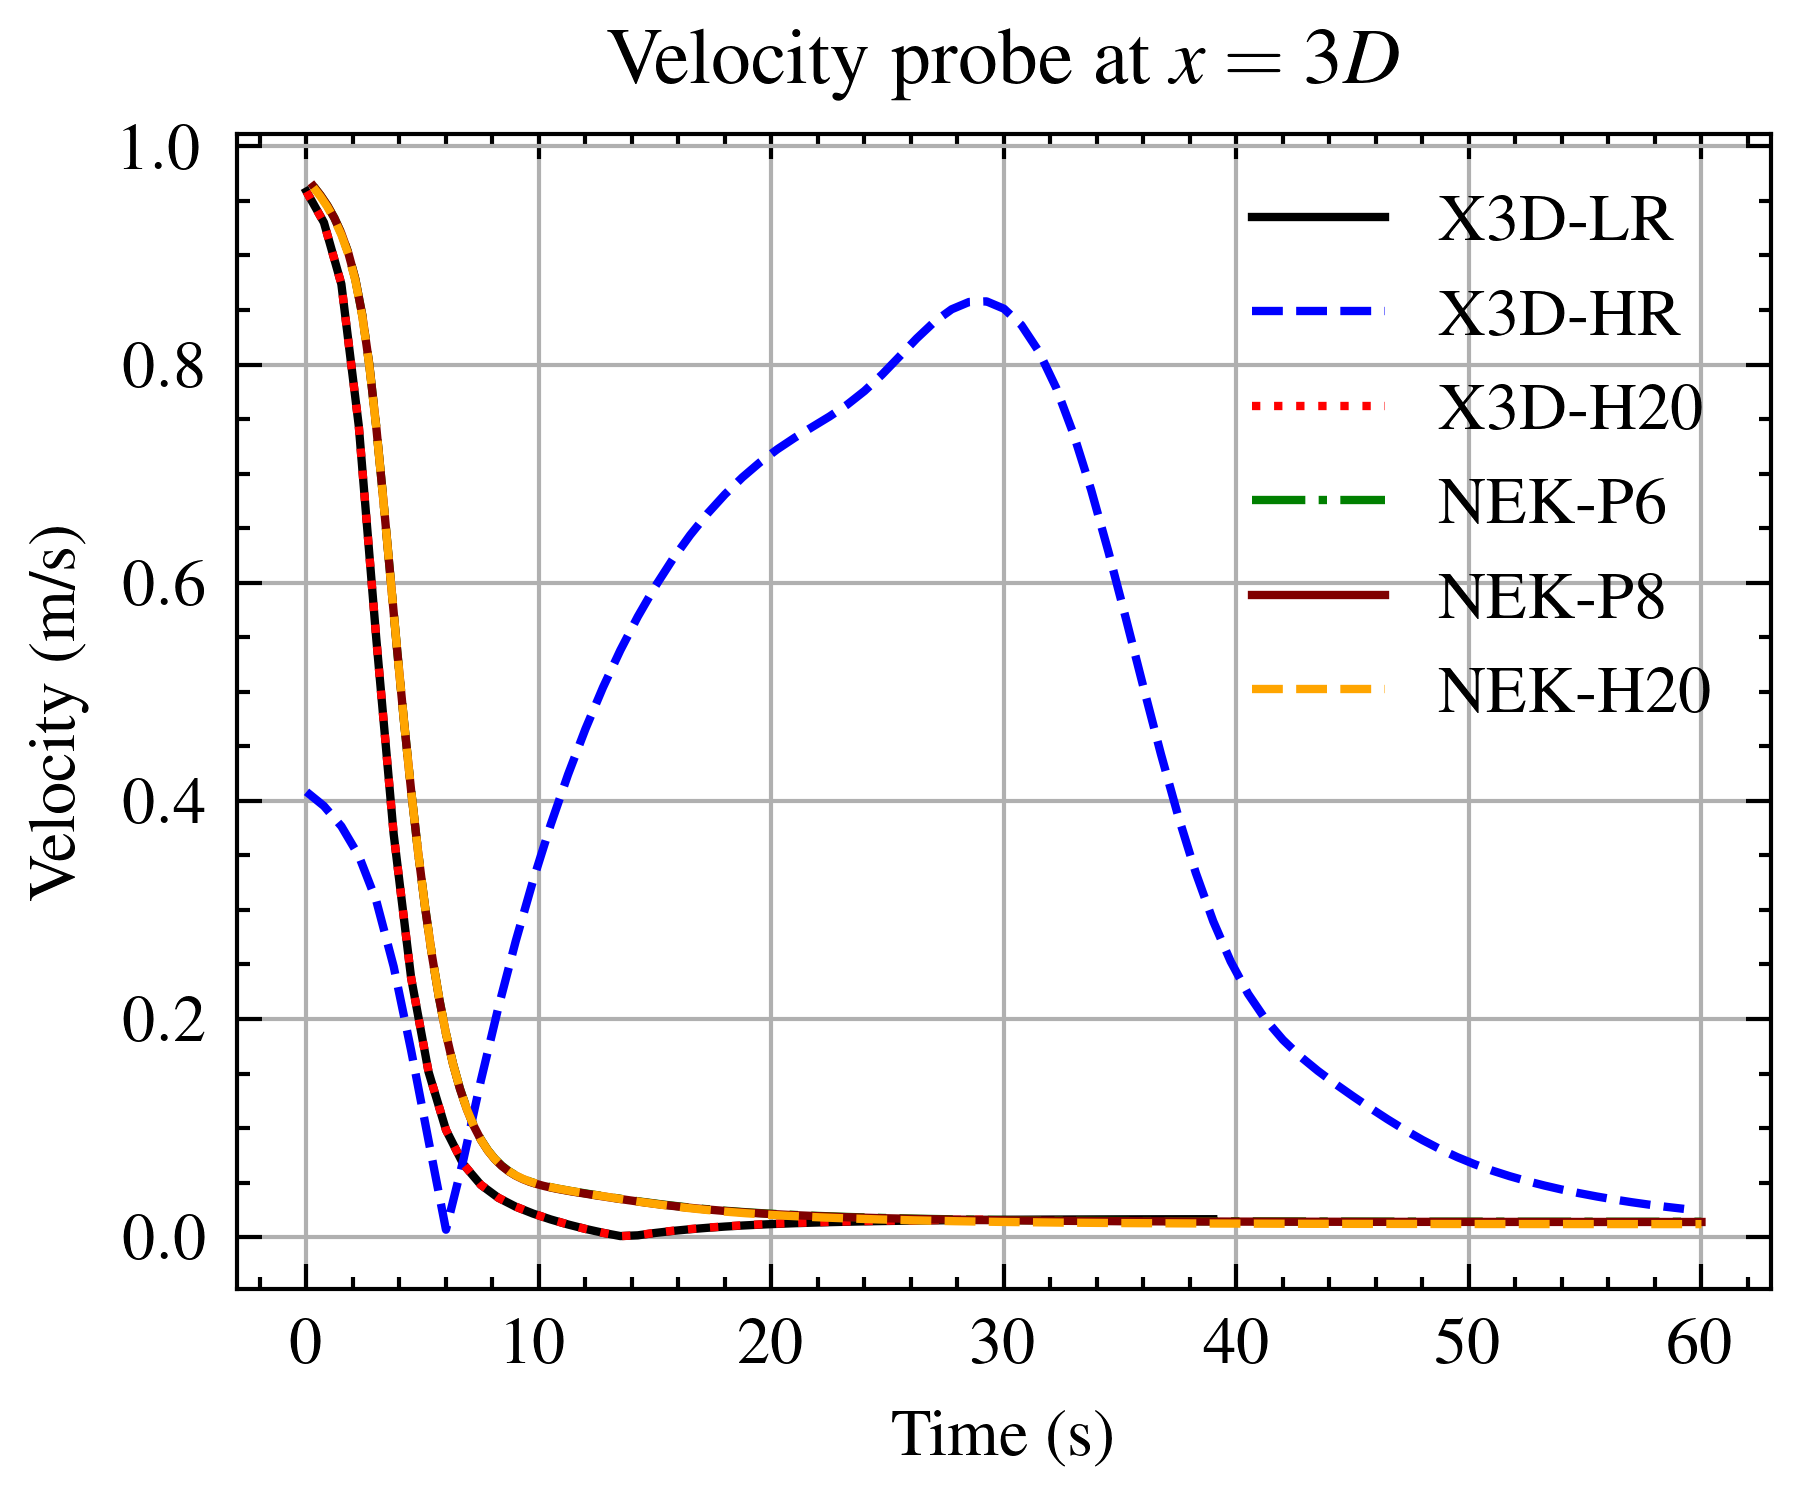
\includegraphics[width=0.55\textwidth]{../ss4dot5.png}
    \caption{Time evolution of velocity magnitude at $x=3 D$ for the different simulations.}
    \label{fig:ss4dot5}
\end{figure}

\noindent In \textbf{Figure \ref{fig:ss3}} and \textbf{Figure \ref{fig:ss4dot5}}, we observe that all the simulations except X3D-HR
reach steady state after $20s$ approximately.
\newpage

\noindent The flow velocity along the X-axis for all the simulations at the last time-step is plotted in \textbf{Figure \ref{fig:xv}}.
Here also we can observe that plots for all the NEK5000 simulation coincide.
\begin{figure}[H]
    \centering
    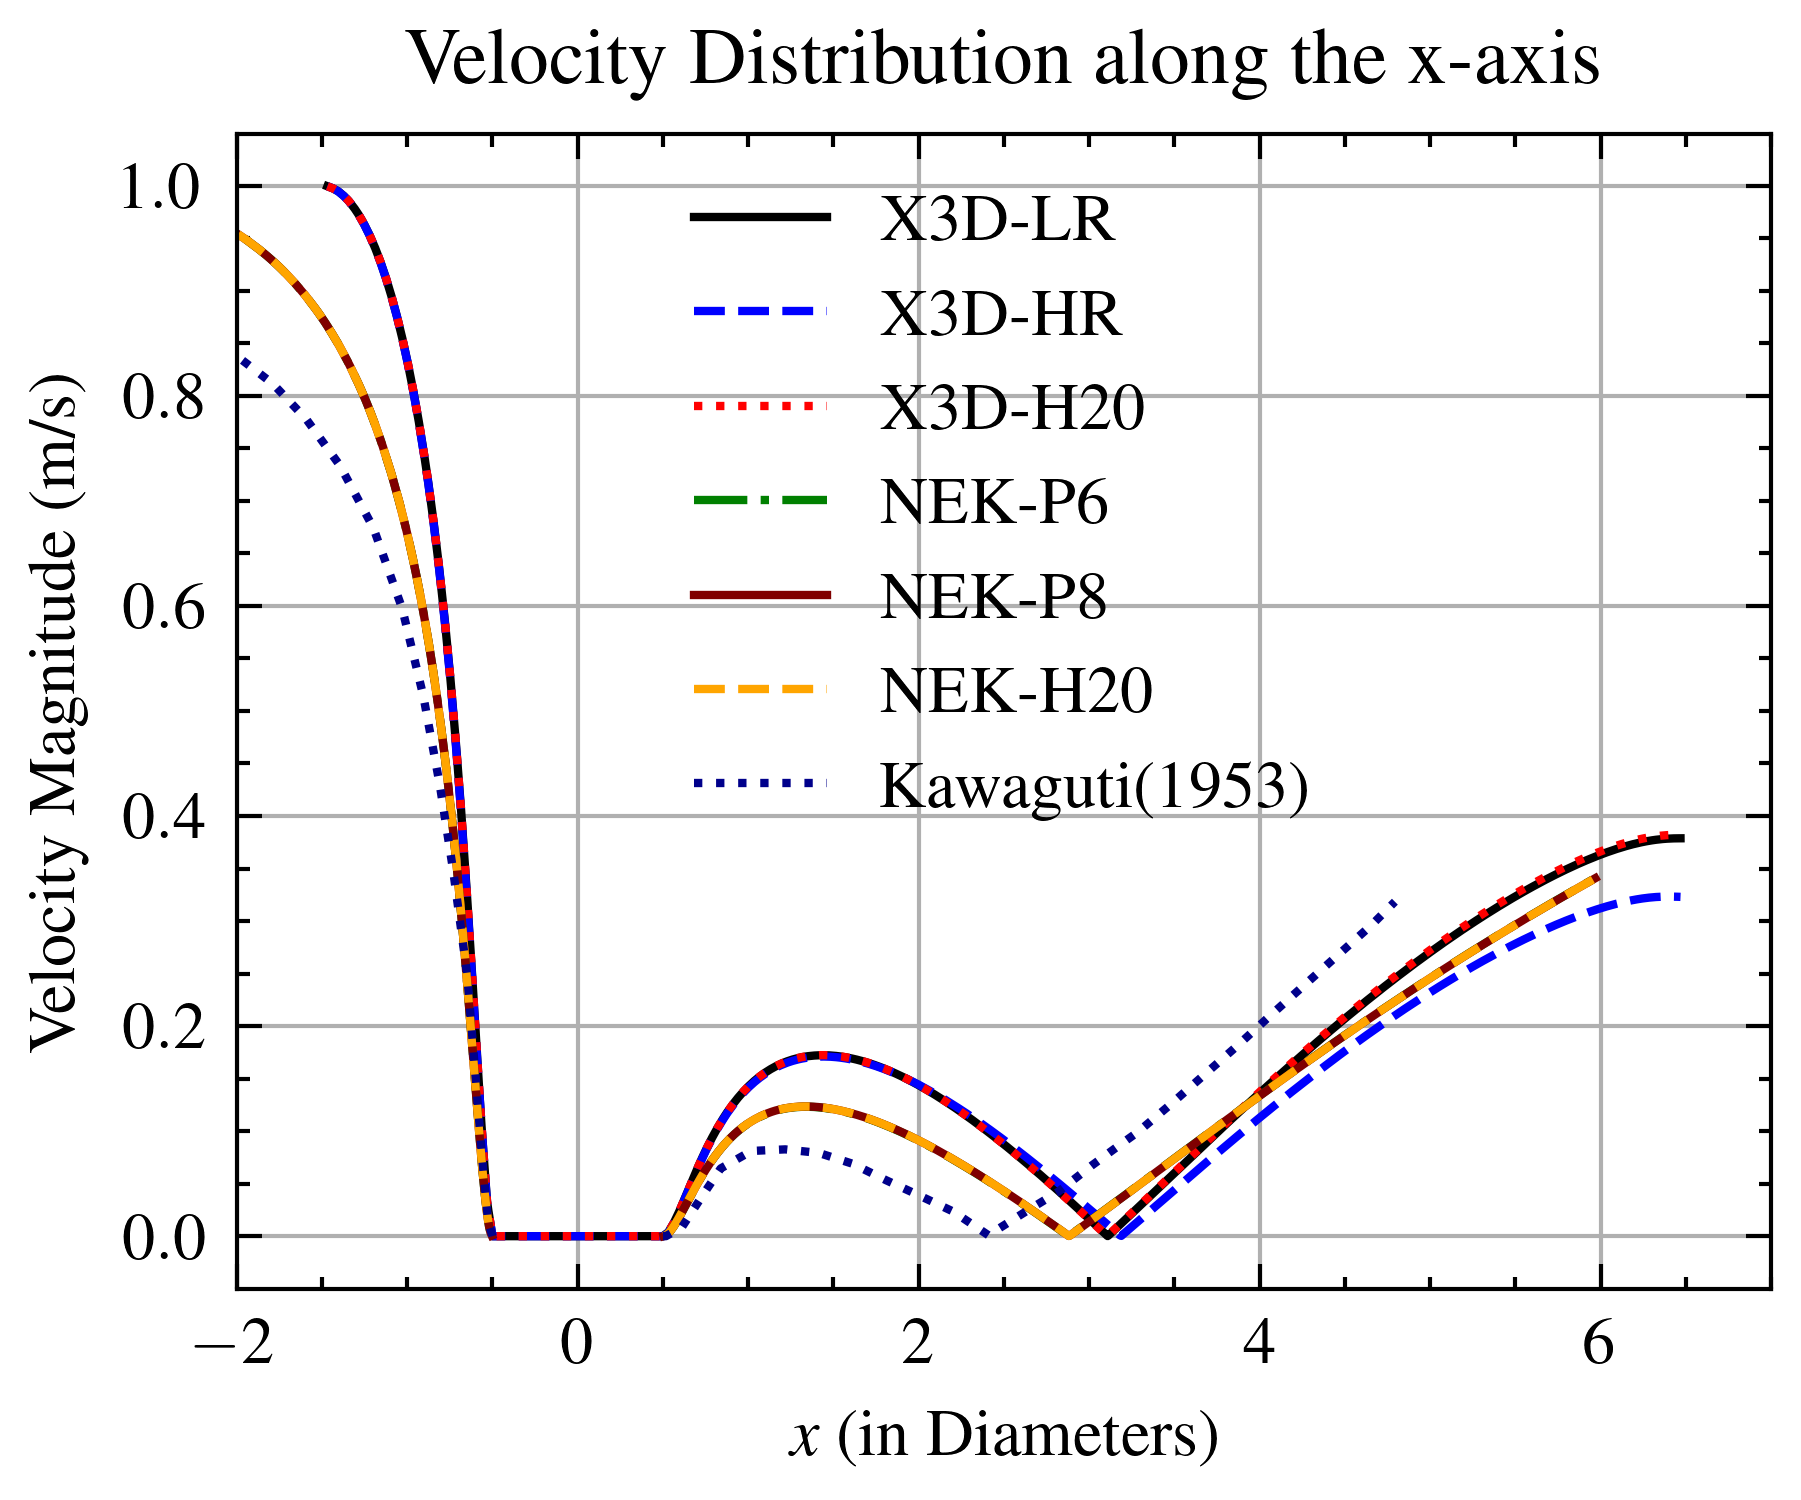
\includegraphics[width=0.7\textwidth]{../xv.png}
    \caption{Varition of velocity along the X-axis after reaching steady-state.}
    \label{fig:xv}
\end{figure}

\subsubsection*{Twin Vortices}
The twin vortices is a flow characteristic of low Re flows around a cylinder such as Re=40. The length of the twin vortices ($L$) and
angle of flow seperation from the cylinder surface ($\theta$) are few of the many flow properties used for validation.
Here, the values of $L$ and $\theta$ obtained by \textbf{Kawaguti} and \textbf{Taneda} are presented in the following table.

\begin{table}[H]
    \centering
    \caption{Twin Vortices length $L$ and the seperation angle $\theta$ used for reference.}
    \begin{tabular}{|c|c|c|}
        \hline
        \textbf{Source} & $\mathbf{L}$ & $\mathbf{\theta}$ \\
        \hline
        Kawaguti (1953) & 1.9 D        & $52.2^{\circ}$    \\
        \hline
        Taneda (1955)   & 2.1 D        & $53^{\circ}$      \\
        \hline
    \end{tabular}
\end{table}

\begin{table}[H]
    \centering
    \caption{Twin Vortices length $L$ and the seperation angle $\theta$ for different simulations.}
    \label{table:tv}
    \begin{tabular}{|c|c|c|}
        \hline
        \textbf{Source} & $\mathbf{L}$ & $\mathbf{\theta}$ \\
        \hline
        X3D-LR          & 2.6 D        & $50.32^{\circ}$   \\
        \hline
        X3D-HR          & 2.65 D       & $54.81^{\circ}$   \\
        \hline
        X3D-H20         & 2.6 D        & $50.8^{\circ}$    \\
        \hline
        NEK-P6          & 2.37 D       & $54.17^{\circ}$   \\
        \hline
        NEK-P8          & 2.37 D       & $54.03^{\circ}$   \\
        \hline
        NEK-H20         & 2.37 D       & $53.77^{\circ}$   \\
        \hline
    \end{tabular}
\end{table}

\begin{figure}[H]
    \centering
    \includegraphics[width=\textwidth]{../tv.png}
    \caption{Twin Vorticies formed behind the cylinder for different simulations.}
    \label{fig:xv}
\end{figure}

\section{Conclusion}
From the above comparison, we observe that NEK5000 simulations are more efficient and accurate in comparison
to the Xcompact3D simulations. The accuracy of the NEK5000 simulations can be improved further by increasing
the number of elements near the cylinder body while keeping the domain big enough such that the
far-field boundary condition is achieved. NEK5000 simulations allow mesh refinement in all directions unlike Xcompact3D
and hence require less number of elements to achieve much better accuracy.
\end{document}
